\chapter{Direction 1: disentangling decoding from belief in LLM advice}
\label{chap:direction1}

%% -----------------------------------------------------------------------
\section{Overview}
\label{sec:d1_overview}

We tested four post-trained large language models on 132 ambiguous
Reddit decision posts under four prompt conditions. Verbalized Sampling
recovered 94--101\% of the entropy gap across all four models. The
remainder of this chapter establishes that this recovery is
mechanism-specific, holds across all four models, and is not explained
by sampling temperature.

\Cref{sec:d1_baseline} documents the baseline entropy gap and its
magnitude. \Cref{sec:d1_hypotheses} frames two competing mechanistic
hypotheses — decoding collapse versus belief collapse — and derives the
diagnostic implication of each. \Cref{sec:d1_vs} presents the Verbalized
Sampling test and its outcome, including the secondary Distribution
Verbalization variant. \Cref{sec:d1_temperature} shows that raising
sampling temperature from 0.7 to 1.2 produces only a fraction of the
entropy recovery achieved by changing output format, ruling out
temperature as the primary driver. \Cref{sec:d1_crossmodel} documents
robustness across the four models and discusses the between-model spread
honestly. \Cref{sec:d1_synthesis} synthesises the evidence and opens the
role-framing question that Chapter 5 addresses.

%% -----------------------------------------------------------------------
\section{Establishing the baseline gap}
\label{sec:d1_baseline}

The forced-choice baseline reveals an entropy gap of striking magnitude
between LLM outputs and the upvote-weighted comment distribution on the
same posts.

\subsection*{Method recap}
\label{subsec:d1_method}

We constructed a corpus of 620 Reddit decision posts spanning education,
career, finance, health, and social subreddits (full pipeline described
in \cref{chap:methodology}). For Direction 1 we retained the 132 posts
whose upvote-weighted human risky ratio fell in [0.20, 0.80] — the
ambiguous subset, where the online community itself was genuinely
divided. We queried four study models (GPT-5, Claude Sonnet 4.6, Mistral
Large 2411, and Llama 4 Maverick) on each post 10 times at temperature
0.7 with a binary forced choice: ``Respond with exactly two words:
\textit{Option A} or \textit{Option B}.'' Option A always mapped to the
riskier option as identified by Step 2 annotation. Outcome variables were
\texttt{llm\_risky\_rate} (fraction of samples choosing the risky
option), \texttt{llm\_entropy} (binary Shannon entropy of that fraction
in nats), \texttt{abs\_gap} ($|$\texttt{llm\_risky\_rate} $-$
\texttt{human\_risky\_ratio}$|$), and KL divergence from the human
distribution.

\subsection*{Results}

Three results characterise the baseline condition.

\textit{Mean entropy gap.} The mean LLM entropy under forced-choice
decoding was 0.046 nats, compared to a human reference entropy of 0.621
nats — a 13-fold gap. Binary entropy is bounded above by $\ln 2 \approx
0.693$ nats, which corresponds to a perfectly balanced 50/50 split. The
human distribution was thus at 90\% of the theoretical maximum, while
LLM entropy was essentially zero. A community that was genuinely
undecided faced advisors who appeared almost certain.

\textit{Mean position gap.} The mean absolute gap was 0.446: LLMs and
the human community differed by 45 percentage points on average in the
direction of advice. This gap is not a calibration drift at the margin
but a structural disagreement about the modal recommendation.

\textit{Effect size.} The Cohen's $d$ for the entropy gap (human minus
LLM) on the ambiguous subset was 3.58, which falls in the range
conventionally labelled extremely large. The gap cannot be explained by
sampling noise.

\begin{figure}[t]
  \centering
  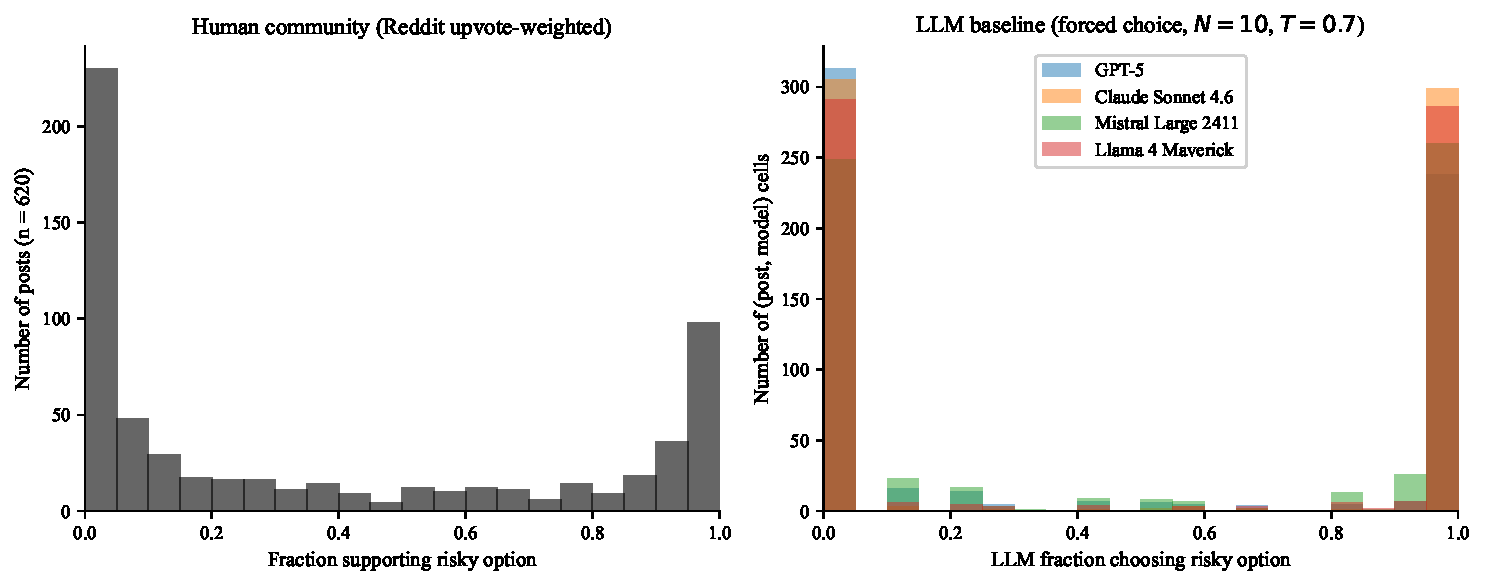
\includegraphics[width=\textwidth]{figures/fig41_distribution_shape/out.pdf}
  \caption{Distribution of human risky ratios and LLM baseline risky
    rates across 132 ambiguous posts. Each bar represents one post;
    the human distribution (left) is centred around 0.5 with spread
    across the full range; the LLM distribution (right) is bimodal at
    0 and 1.}
  \label{fig:d1_histogram}
\end{figure}

The baseline reflects the upvote-weighted distribution of vocal
commenters on five decision-oriented subreddits, not a general human
population \citep{sachdeva-2025-aita}. The same caveat applies
throughout this chapter: our alignment target is community consensus as
expressed through Reddit's voting mechanism, not universal human
preference. The finding nonetheless mirrors a closely analogous result
in moral judgment, where \citet{russo-2026-pluralistic} documented a
comparable collapse on moral-dilemma posts from the same platform.

\Cref{tab:d1_conditions} summarises the four conditions that the
remainder of this chapter tests.

\begin{table}[t]
  \centering
  \caption{Mean entropy, absolute gap, and KL divergence per condition,
    averaged across four models and 132 ambiguous posts. Human reference
    entropy is 0.621 nats throughout.}
  \label{tab:d1_conditions}
  \begin{tabular}{lcccc}
    \toprule
    Condition & $\bar{H}_{\text{LLM}}$ & $\overline{\textit{abs\_gap}}$
              & $\overline{\text{KL}}$ & Recovery \\
    \midrule
    Baseline (forced, $T{=}0.7$)         & 0.046 & 0.446 & 2.378 & — \\
    High-temperature (forced, $T{=}1.2$) & 0.108 & 0.430 & 2.116 & 10.7\% \\
    Distribution Verbalization (DV)      & 0.553 & 0.233 & 0.216 & 88.3\% \\
    Verbalized Sampling (VS)             & 0.608 & 0.210 & 0.161 & 97.9\% \\
    \bottomrule
  \end{tabular}
\end{table}

%% -----------------------------------------------------------------------
\section{Two competing hypotheses}
\label{sec:d1_hypotheses}

The baseline gap admits two qualitatively different explanations with
opposite deployment implications.

\textbf{H$_{\text{decoding}}$ (Decoding collapse).} The model's internal
belief distribution over the two options is broad, but the forced-choice
sampling process at temperature 0.7 systematically discards this breadth,
producing a near-deterministic output. Under this hypothesis, the collapse
is an artifact of the output interface; the model's underlying knowledge
of pluralism is intact. The fix is a prompt-level change that permits the
model to express a distribution rather than commit to a single token.

\textbf{H$_{\text{belief}}$ (Belief collapse).} The model's internal
belief distribution is itself collapsed — reinforcement learning from
human feedback has compressed the probability mass over advice options
into a single modal answer \citep{kirk-2024-rlhf-diversity}. A
theoretical mechanism for this compression is the typicality bias
identified by \citet{chung-2025-soft-preference}: the KL regulariser in
PPO pushes the reward-maximising policy toward modal completions,
systematically discounting minority-but-admissible answers. Under this
hypothesis, the collapse is intrinsic to the model; no prompt-level
intervention can recover pluralism without retraining on more diverse
preference data.

The deployment implications of the two hypotheses are distinct. If
H$_{\text{decoding}}$ is correct, existing frontier models already
encode the pluralism that aligned advice requires, and the fix costs
one line of a prompt. If H$_{\text{belief}}$ is correct, the fix
requires new preference data, retraining, or architectural changes
\citep{ouyang-2022-instructgpt} — an enterprise orders of magnitude
more expensive.

\textit{Diagnostic logic.} Verbalized Sampling provides a clean test
\citep{zhang-2025-verbalized-sampling}. We ask the model to output a
probability distribution over the two options — ``P(Option A) = 0.XX,
P(Option B) = 0.XX'' — rather than committing to a single choice. If
H$_{\text{decoding}}$ is true, this format change should allow the model
to express its full internal distribution, recovering most or all of the
entropy gap. If H$_{\text{belief}}$ is true, the internal distribution
is peaked regardless of how the question is asked; verbalized output
should therefore show entropy close to the forced-choice baseline.

%% -----------------------------------------------------------------------
\section{The Verbalized Sampling test}
\label{sec:d1_vs}

Verbalized Sampling produced near-complete entropy recovery, decisively
favoring the decoding-collapse hypothesis.

\subsection*{Manipulation}

Each post was presented with the same body text and the same Option A /
Option B labelling as in the baseline. The format instruction was
replaced with: ``Output ONLY the two probability lines below, in this
exact format. P(Option A) = 0.XX, P(Option B) = 0.XX.'' We sampled each
model $N{=}3$ times at temperature 0.7 with a maximum of 200 tokens.
Responses were parsed by a strict regular expression that required
explicit P(A) and P(B) tokens; those that summed within [0.90, 1.10]
were renormalised; those outside that range were logged as parse failures
and excluded from analysis. The Distribution Verbalization (DV) variant
asked instead: ``Among advice-givers on /r/\{subreddit\} who saw a post
like this, what fraction would recommend Option A vs Option B?'' — making
the framing descriptive rather than personal, otherwise identical.

\subsection*{Headline results}

The mean LLM entropy under VS was 0.608 nats, compared to 0.046 nats at
baseline and 0.621 nats for the human reference (see
\cref{tab:d1_conditions}). The mean absolute gap fell from 0.446 to
0.210. Recovery, defined as $(H_{\text{VS}} - H_{\text{baseline}}) /
(H_{\text{human}} - H_{\text{baseline}})$, was 94--101\% across the four
models (\cref{sec:d1_crossmodel}). The result was statistically robust:
paired bootstrap ($n{=}525$ post--model pairs, 10\,000 resamplings) gave
$\Delta = -0.235$, 95\% CI $[-0.250, -0.220]$, $p_{\text{fdr}} <
0.001$.

\begin{figure}[t]
  \centering
  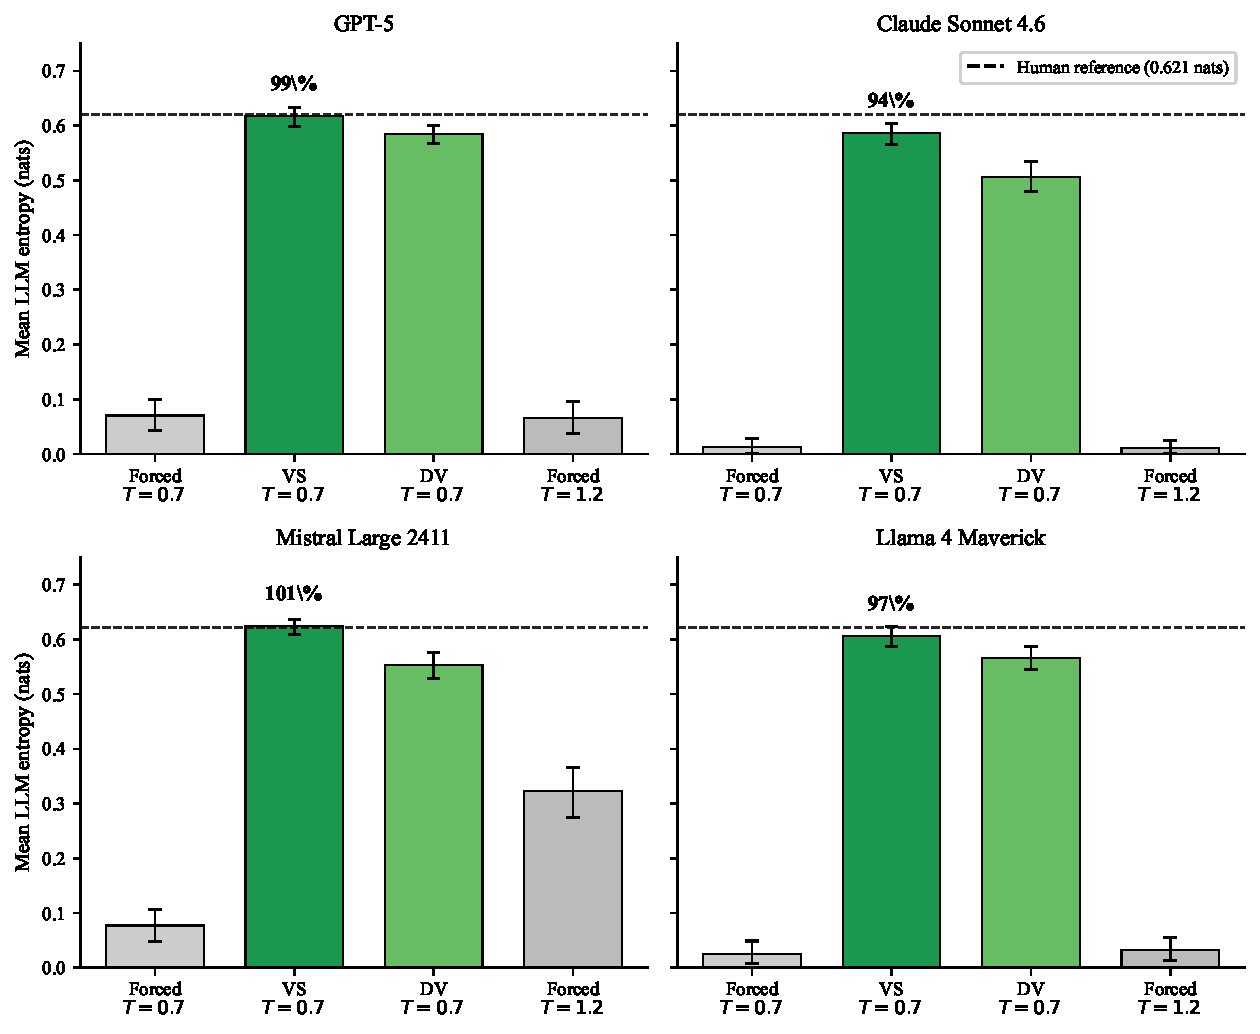
\includegraphics[width=\textwidth]{figures/fig42_d1_entropy_by_model_condition/out.pdf}
  \caption{Mean LLM entropy per condition for each of the four study
    models. The dashed horizontal line marks human reference entropy
    (0.621 nats). Verbalized Sampling (VS) approaches the human
    reference in all four models; high-temperature forced choice (hight)
    does not.}
  \label{fig:d1_entropy_panels}
\end{figure}

This result extends the finding of \citet{zhang-2025-verbalized-sampling}
— who demonstrated entropy recovery on creative writing, joke generation,
and donation amounts — to binary forced-choice advice on personal
decisions. The recovery is not only statistically significant but
practically complete: a model that recovers near-human entropy under VS
while producing near-zero entropy under forced choice cannot have a
collapsed internal belief.

\subsection*{Distribution Verbalization (secondary condition)}

DV recovered 88\% of the entropy gap on average (mean entropy 0.553
nats, abs\_gap 0.233). The gap between VS and DV was small but
significant: $\Delta_{\text{VS-DV}} = -0.023$, 95\% CI $[-0.033,
-0.013]$, $p_{\text{fdr}} < 0.001$. We attribute this difference to the
descriptive framing in DV (``what would the community recommend'') versus
VS's direct probability elicitation: the descriptive prompt asks the
model to reason about a third-party distribution rather than express its
own, introducing one layer of indirection. The contrast between DV and
VS will be revisited in the role-framing analysis of
\cref{chap:direction2}, where we hold output format fixed and manipulate
descriptive versus prescriptive framing directly.

\subsection*{KL divergence as a triangulating measure}

Replacing the symmetric abs\_gap measure with the directional
KL divergence $\text{KL}(\text{human} \| \text{LLM})$ yields
the same qualitative pattern. Baseline KL was 2.378 nats; VS KL
was 0.161 nats, a 14.8-fold reduction (\cref{tab:d1_conditions}).
DV reduced KL to 0.216 nats. The KL results confirm that VS brings
the LLM distribution close to the human target in shape, not merely
in its first moment.

Per-cell estimates from VS and DV used $N{=}3$ samples, which is noisier
than the $N{=}10$ baseline. Across 132 posts and 4 models the aggregate
comprises 528 cells and 1,584 observations; the pooled signal is robust
despite per-cell noise.

%% -----------------------------------------------------------------------
\section{Ruling out temperature}
\label{sec:d1_temperature}

If the collapse observed at baseline were driven by the low sampling
temperature, simply raising the temperature should produce entropy
comparable to VS — but it does not.

\subsection*{Design}

The high-temperature (hight) condition used the exact baseline prompt
(forced binary choice) but set $T{=}1.2$ and drew $N{=}20$ samples per
post per model, giving a finer-grained estimate of the choice
distribution under higher stochasticity.

\subsection*{Results}

Pooled across models, high-temperature entropy was 0.108 nats —
0.062 nats above baseline, but 0.500 nats below VS. The mean abs\_gap
fell only from 0.446 to 0.430. The entropy gain was statistically
detectable ($\Delta = -0.016$, 95\% CI $[-0.026, -0.005]$,
$p_{\text{fdr}} = 0.004$, two asterisks) but practically negligible:
Cohen's $d < 0.10$. VS produced 9.1 times more entropy gain than
the high-temperature control (relative to baseline), despite using a
lower temperature (0.7 versus 1.2).

The high-temperature effect was, however, strongly heterogeneous across
models. GPT, Claude, and Llama showed near-zero recovery (mean entropy
0.066, 0.011, and 0.033 nats respectively — essentially identical to
their baseline values). Mistral was the exception: high-temperature
entropy reached 0.323 nats, corresponding to 45\% entropy recovery.
This cross-model heterogeneity has an important implication. Even for
the model that responded most strongly to temperature, VS recovered
100.5\% of the entropy gap at a lower temperature. Temperature therefore
explains at most a fraction of the Mistral entropy recovery, and none of
the GPT, Claude, or Llama recovery.

\textit{Conceptual conclusion.} The relevant lever is output format
(single-token versus probability distribution), not sampling temperature
applied to that format. \citet{renze-2024-temperature} showed that
temperature has limited effect on accuracy in language models more
broadly; our result extends that null to distributional alignment on
advice tasks. \citet{zhang-2025-verbalized-sampling} explicitly
distinguished their method from temperature-based diversity interventions
on the same grounds.

One might object that a higher temperature still (e.g., $T{=}2.0$) could
close the remaining gap. This is implausible for two reasons. First, at
$T{=}1.2$ the parse failure rate for high-temperature forced-choice
responses was 2.6\%, compared to 0.8\% at baseline — indicating that the
format is already beginning to degrade. Higher temperatures produce
noise rather than pluralism, a qualitatively different phenomenon.
Second, Mistral at $T{=}1.2$ showed 45\% recovery; VS at $T{=}0.7$
showed 100.5\%. The ceiling argument requires implausibly large
temperature increases to close a gap that a format change closes
completely.

%% -----------------------------------------------------------------------
\section{Cross-model robustness}
\label{sec:d1_crossmodel}

The decoding-collapse pattern holds across four post-trained models that
differ in training procedure, scale, and developer, indicating a property
of the post-training paradigm rather than of any individual model.

\Cref{tab:d1_model_breakdown} reports the full per-model results. All
four models showed greater than 94\% entropy recovery under VS. The
entropy gap at baseline was large for every model ($d > 2.5$ in each
case): GPT's baseline entropy was 0.070 nats, Claude's 0.013 nats,
Mistral's 0.077 nats, and Llama's 0.026 nats, compared to the human
reference of 0.621 nats throughout.

\begin{table}[t]
  \centering
  \caption{Per-model entropy and recovery by condition. Recovery is
    $(H_{\text{cond}} - H_{\text{baseline}}) /
    (H_{\text{human}} - H_{\text{baseline}}) \times 100\%$.
    Human reference entropy: 0.621 nats.}
  \label{tab:d1_model_breakdown}
  \begin{tabular}{llcccr}
    \toprule
    Model & Condition & $H_{\text{LLM}}$ & $\overline{\textit{abs\_gap}}$
          & $\overline{\text{KL}}$ & Recovery \\
    \midrule
    GPT     & Baseline  & 0.070 & 0.428 & 2.193 & — \\
            & Hight     & 0.066 & 0.434 & 2.238 & $-0.8\%$ \\
            & DV        & 0.585 & 0.212 & 0.166 & 93.5\% \\
            & VS        & 0.617 & 0.197 & 0.138 & 99.3\% \\
    \midrule
    Claude  & Baseline  & 0.013 & 0.480 & 2.680 & — \\
            & Hight     & 0.011 & 0.484 & 2.690 & $-0.2\%$ \\
            & DV        & 0.506 & 0.264 & 0.292 & 81.1\% \\
            & VS        & 0.586 & 0.227 & 0.180 & 94.2\% \\
    \midrule
    Mistral & Baseline  & 0.077 & 0.432 & 2.210 & — \\
            & Hight     & 0.323 & 0.352 & 1.135 & 45.2\% \\
            & DV        & 0.553 & 0.243 & 0.221 & 87.6\% \\
            & VS        & 0.624 & 0.205 & 0.137 & 100.5\% \\
    \midrule
    Llama   & Baseline  & 0.026 & 0.444 & 2.429 & — \\
            & Hight     & 0.033 & 0.450 & 2.408 & 1.2\% \\
            & DV        & 0.566 & 0.214 & 0.188 & 90.8\% \\
            & VS        & 0.606 & 0.213 & 0.188 & 97.5\% \\
    \bottomrule
  \end{tabular}
\end{table}

Three observations warrant discussion.

\textit{All four models showed greater than 90\% VS recovery.} The
finding is not a single-model artifact. GPT (99.3\%), Claude (94.2\%),
Mistral (100.5\%), and Llama (97.5\%) all converged toward the human
reference when permitted to express a probability distribution. The
consistency across models trained by different organisations with
different RLHF pipelines \citep{ouyang-2022-instructgpt, bai-2022-constitutional} is the scientifically decisive fact: decoding
collapse appears to be a property of the post-training paradigm, not of
any particular implementation.

\textit{Mistral exceeded 100\% recovery.} A recovery above 100\% implies
that Mistral's VS distribution was slightly broader than the human
reference distribution. Two interpretations are compatible with the data.
First, Mistral's post-training may apply less aggressive RLHF compression
than the other three models, leaving internal beliefs more diffuse; when
the format permits expression of that diffuseness, they overshoot the
human reference slightly. Second, the 0.5 percentage-point overshoot is
within the bootstrap 95\% confidence interval of the human reference
itself, and may reflect sampling noise in the $N{=}3$ VS draws per cell.
We do not resolve this question here; it merits investigation with larger
per-cell sample sizes in future work.

\textit{Claude's 94.2\% recovery was the lowest.} Constitutional AI
training \citep{bai-2022-constitutional} may produce more prescriptive
priors — the model is trained to give a single helpful answer, which
could resist distributional output even when explicitly asked. Claude's
recovery is, however, still substantially above 90\%, so the
interpretation remains that decoding is the dominant driver. The precise
contribution of Constitutional AI is speculative and left for future work.

The 7.3 percentage-point spread across models (94.2\% to 100.5\%) is
smaller than the 95\% confidence interval around any individual model's
estimate; the between-model variation is not statistically distinguishable
from noise at these sample sizes. The robust claim is the consistency
across models, not the ordering within the spread \citep{kirk-2024-rlhf-diversity}.

\todo{fig 4.3: per-model VS recovery rates (99, 94, 101, 98 per cent)
  with 95\% CI from bootstrap, as a four-bar horizontal chart. Optional
  — include if not redundant with \cref{fig:d1_entropy_panels}.}

%% -----------------------------------------------------------------------
\section{Interim synthesis and forward link}
\label{sec:d1_synthesis}

Direction 1 establishes that the entropy gap is recoverable through an
interface-level intervention, but two questions remain open.

\textit{Is the role of the LLM a separate driver?} The DV condition hinted
at a small descriptive effect: asking the model to describe community
preferences (rather than express its own) recovered 88\% versus VS's
98\%, a 10 percentage-point difference that was statistically significant
($p_{\text{fdr}} < 0.001$). However, DV changed two things simultaneously
— the framing of the question and the output format — confounding role
with format. Chapter 5 isolates role framing by holding output format
fixed at single-token forced choice and varying only whether the model is
cast as a personal advisor, a predictive oracle, or a first-person agent.

\textit{Does the finding generalise beyond the ambiguous subset?} The 132
posts analysed here were filtered to human\_risky\_ratio $\in [0.20,
0.80]$, by construction the posts where human opinion was most divided.
Chapter 5 tests role-framing effects across the full 620-post corpus,
covering a broader range of consensus levels and providing a more
general view of the alignment gap.

The decoding-collapse hypothesis is now supported on four independent
grounds. First, mean entropy rose from 0.046 to 0.608 nats under VS —
a 13-fold increase with the same underlying model. Second, the recovery
rate was 94--101\% across four models from different organisations and
training pipelines. Third, raising sampling temperature from 0.7 to 1.2
produced only 10.7\% entropy recovery in the same forced-choice format,
compared to VS's 97.9\% at the lower temperature; the decisive variable
is the format constraint, not the decoding temperature. Fourth, the
VS-versus-baseline difference was statistically robust across multiple
comparison correction ($p_{\text{fdr}} < 0.001$ after Benjamini-Hochberg
adjustment over 11 comparisons). The belief-collapse hypothesis is
provisionally rejected for these four models: a model whose internal
distribution is genuinely collapsed cannot recover near-human entropy
when a different output format is used.

Having identified output format as the primary lever, we now ask whether
role framing — a manipulation that holds output format fixed but varies
the LLM's assigned epistemic role — produces an analogous, additive, or
negligible effect.
